\documentclass[tikz]{standalone}
\usetikzlibrary{automata,positioning}
\begin{document}

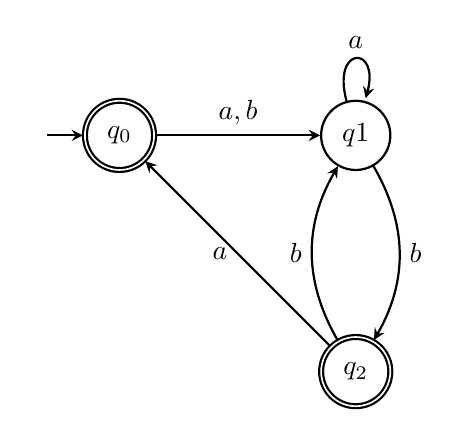
\begin{tikzpicture}[>=stealth,node distance=3cm,on grid,auto, thick, initial text=] 
  \node[state,initial,accepting] (q_0)   {$q_0$}; 
  \node[state]         (q_1) [right=3cm of q_0] {$q1$};
  \node[state,accepting]  (q_2) [below=3cm of q_1] {$q_2$};

  \path[->]            (q_0) edge  node {$a,b$} (q_1)
                       (q_1) edge [loop above] node [above] {$a$} (q_1)
                             edge [bend left] node[right] {$b$} (q_2)

(q_2) edge node [left] {$a$} (q_0)

edge [bend left] node [left] {$b$} (q_1);
                             
\end{tikzpicture}
\end{document}